%!TEX root = ../template.tex
\chapter{Related Work (10/02/2021)}\label{cha:related-work}

\section{Language Preprocessors}\label{sec:lang-preprocessors}
Language preprocessors are a mechanism which runs during compilation,
some languages will apply the preprocessor during different compilation stages while others will only apply the preprocessor in a single stage.

% \subsection{C and C++}\label{sec:lang-preprocessors:c-cpp}

\subsection{OCaml}\label{sec:lang-preprocessors:ocaml}

The OCaml ecosystem currently uses OCaml \gls{PPX},
however, previous to version 4.02, OCaml made use of \gls{p4}.

We briefly review both \gls{p4} and \gls{PPX}.

\subsubsection*{Camlp4}\label{sec:lang-preprocessors:ocaml:p4}

Camlp4 is a parsing library which provides extensible grammars,
its main goal is to allow users to extend OCaml syntax,
Camlp4 is also able to redefine the core syntax,
OCaml even introduced a revised syntax~\autocite{Rauglaudre2003} to enable Camlp4.

The library has been deprecated due to being confusing to users and tools alike.
Users were required to learn the revised OCaml syntax which complicates the development process.
These criticisms are found throughout documents which discuss Camlp4~\autocite{Whitequark2014}.

In a nutshell, the Camlp4 library would allow developers to develop an extension syntax,
when the compiler would pass the source code as text to the preprocessor,
which, in turn would generate valid OCaml source code.

\subsubsection*{PPX}\label{sec:lang-preprocessors:ocaml:ppx}

\subsection{Java}\label{sec:lang-preprocessors:java}

As other languages, Java is also capable of source code processing during compile time,
we review two existing approaches, annotations and the ExtendJ compiler.

\subsubsection*{Java Annotation Processor}\label{sec:lang-preprocessors:java:annotation}

Java annotations were first introduced in Java 5 \autocite{JSR269},
they are a form of metadata which can be added to Java source code.
Annotations can be used in conjunction with several components of the Java language,
such as classes, interfaces, documentation and others.
These are processed by build-time tools or by run-time libraries to achieve new semantic effects,
a popular example of such library would be the compile-time dependency injection framework Dagger 2~\autocite{Dagger2}.

% \paragraph{Annotation Syntax} is simple: every annotation starts with an \texttt{@} and is followed by an identifier, optionally, the annotation can take parameters.

% \begin{minted}{java}
% @Annotation
% \end{minted}

\subsubsection*{ExtendJ \& JastAdd}\label{sec:lang-preprocessors:java:extendj}

\subsection{Kotlin}\label{sec:lang-preprocessors:kotlin}

\subsubsection*{Kotlin Compiler Plugins}\label{sec:lang-preprocessors:kotlin:annotation}


\section{Rust Macros}\label{sec:rust-macros}

Just like its predecessors, C \& C++, Rust offers macros as part of the language.
In essence, Rust macros are just like other languages macro's, running during compile-time to generate code.
In Rust, macros refer to a family of features (see \autoref{fig:rust-macro-family}),
\emph{declarative} macros and \emph{procedural} macros.

\begin{figure}
    \centering
    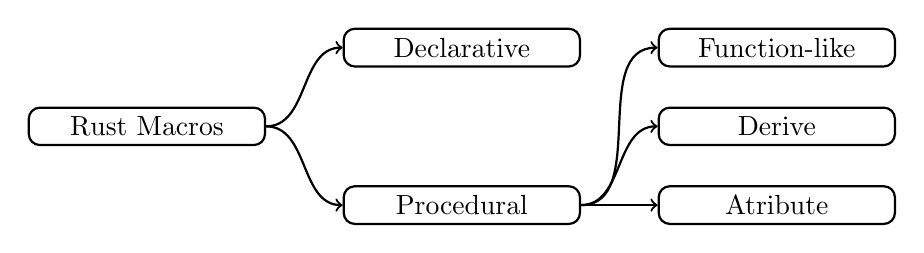
\begin{tikzpicture}
        \tikzset{
            member/.style={
                    rectangle,
                    rounded corners,
                    draw=black,
                    thick,
                    minimum width=3cm,
                },
            connection/.style={->, thick},
        }
        % \draw (0, -2) grid (6, 2);
        \node[member] (root) at (-1, 0) {Rust Macros};
        \node[member] (decl) at (3, 1) {Declarative};
        \node[member] (proc) at (3, -1) {Procedural};
        \node[member] (func) at (7, 1) {Function-like};
        \node[member] (derv) at (7, 0) {Derive};
        \node[member] (attr) at (7, -1) {Atribute};
        \draw[connection] (root) edge[out=0, in=180] (proc);
        \draw[connection] (root) edge[out=0, in=180] (decl);
        \draw[connection] (proc) edge[out=0, in=180] (func);
        \draw[connection] (proc) edge[out=0, in=180] (derv);
        \draw[connection] (proc) edge[out=0, in=180] (attr);
    \end{tikzpicture}
    \caption{Rust macro's family tree}
    \label{fig:rust-macro-family}
\end{figure}

\subsection{Declarative Macros}\label{sec:rust-macros:decl}

Declarative macros (also known as \emph{macros-by-example}) can be declared with \texttt{macro\_rules!}
and are called with function syntax (see \autoref{lst:rust-macro-rules}).

\begin{displayquote}[{\autocite[Section 3.1]{RustRef2021}}]
    Each macro by example has a name, and one or more rules.
    Each rule has two parts: a matcher, describing the syntax that it matches, and a transcriber,
    describing the syntax that will replace a successfully matched invocation.
    Both the matcher and the transcriber must be surrounded by delimiters.
    Macros can expand to expressions, statements, items
    (including traits, impls, and foreign items), types, or patterns.
\end{displayquote}

\paragraph{Transcribing.}
When a macro is invoked, the macro expander loops through the declared rules, transcribing the first successful match.
It transcribes the first successful match; if this results in an error, then future matches are not tried.
An error is thrown if the compiler cannot determine unambiguously how to parse the macro
\autocite[Section 3.1 - Transcribing]{RustRef2021}.

\paragraph{Metavariables.}
To specify a macro a user first declares a pattern which will match a given form of syntax.
\emph{Metavariables} are used to achieve such goal,
they are declared with “\texttt{\$ \keyword{name} : \keyword{fragment-specifier}}” in the macro matcher and
can match thirteen different kinds of syntax fragments \autocite[Section 3.1 - Metavariables]{RustRef2021}.
In \autoref{lst:rust-macro-rules}, the metavariable \texttt{n} is of kind \texttt{literal}
which will match literals such as \texttt{'E'}, \texttt{"Elite"} and \texttt{420} \autocite[Section 8.2.1]{RustRef2021}.

\paragraph{Repetitions} are indicated by placing the tokens to be repeated inside \texttt{\$(...)},
followed by a repetition operator, optionally with a separator token between.
This is valid both for the matcher and the transcriber.
Repetition operators are the same as the regular expression ones:
\begin{compactitem}
    \item \texttt{*} — indicates zero or more repetitions.
    \item \texttt{+} — indicates at least one repetition.
    \item \texttt{?} — indicates zero or one repetition.
\end{compactitem}

\paragraph{Hygiene} works by attaching an invisible \emph{syntactic context} to all identifiers \autocite{Wirth2021}.
Identifiers are compared over two pieces of information,
the \emph{textual value} and their \emph{syntactic context}.
The textual value consists of the variables name (e.g. \texttt{four}),
the syntactic context is a kind of scope added to variables declared inside the macro.
This is done to keep the macro declared variables from interfering with existing ones.

When expanding a declarative macro\footnotemark variables declared inside the macro belong in a different scope,
consider the macro declared in \autoref{lst:rust-macro-hygiene:declaration} and
the respective expansion in \autoref{lst:rust-macro-hygiene:expansion}.
As illustrated by \autoref{lst:rust-macro-hygiene:expansion},
line 2 is considered to be in a different context than the rest of the expanded code.
This will rightfully raise an error (shown in \autoref{lst:rust-macro-hygiene:error}),
since line's 3 \texttt{a} will not exist due to not being in the same syntactic context as line 2.

\footnotetext{
    The same mechanism does not apply to procedural macros, which are not hygienic.
    Their output will interfere with existing code if precautions are not taken \autocite{Koxiaet2020}.
}

\begin{listing}
    \centering
    \begin{minted}{Rust}
macro_rules! say_hello {
    ($n:literal) => {
        for 0..$n {
            println!("Hello, world!");
        }
    }
}
fn main() {
    say_hello!(5);
}
    \end{minted}
    \caption{Example \texttt{macro\_rules!} usage.
        When executed, the code above will print “\texttt{Hello, world!}” five times.}
    \label{lst:rust-macro-rules}
\end{listing}


\begin{listing}
    \begin{minted}{Rust}
macro_rules! using_a {
    ($e:expr) => {
        {
            let a = 42;
            $e
        }
    }
}
let four = using_a!(a / 10);
    \end{minted}
    \caption{
        Definition of the \texttt{using\_a} macro and usage.
        The macro simply declares a variable \texttt{a},
        set to 42 and then writes an expression which was passed in.
    }
    \label{lst:rust-macro-hygiene:declaration}
\end{listing}

\begin{listing}
    \begin{minted}[highlightlines=2,highlightcolor=blue!10]{Rust}
let four = {
    let a = 42;
    a / 10
};
    \end{minted}
    \caption{
        \autoref{lst:rust-macro-hygiene:declaration} line 9's macro expansion.
        Declarations with a blue background will be placed in a different \emph{scope} than the others,
        thus the \texttt{a} for lines 2 and 3 will not be considered the same.
    }
    \label{lst:rust-macro-hygiene:expansion}
\end{listing}

\begin{listing}
    \begin{minted}{text}
error[E0425]: cannot find value `a` in this scope
  --> src/main.rs:13:21
   |
 9 | let four = using_a!(a / 10);
   |                     ^ not found in this scope
    \end{minted}
    \caption{
        The expansion in \autoref{lst:rust-macro-hygiene:expansion} will result in an error during compile time
        since the \texttt{a}s in line 2 and 3 are considered to belong to different contexts.
    }
    \label{lst:rust-macro-hygiene:error}
\end{listing}

\subsection{Procedural Macros}\label{sec:rust-macros:proc}
Rust also has another macro mechanism, \emph{procedural macros},
these can take three forms: \emph{function-like macros}, \emph{derive macros} and \emph{attribute macros}.
In a nutshell, procedural macros allow users to run code at compile time, consuming and producing Rust syntax.

\subsubsection*{Function-like Macros}
Function-like macros and declarative macros are similar regarding invocation, being indistinguishable from each other,
and output, completely replacing the original call.
However, the similarities stop there as their implementation methods are completely different.

\paragraph{Definition.}
Function-like macros are defined by a public function with the \texttt{proc\_macro} attribute and
a signature of type \texttt{(TokenStream) -> TokenStream}.
Everything contained inside the call delimeters of the macro invocation is input to the function,
as previously referred, the output will completely replace the macro call.

\paragraph{Domain Specific Languages.}
While the macros discussed next also provide their contribution for domain specific languages in Rust,
function-like macros provide the necessary tools to write an embedded DSL.
The Rust ecosystem developers have developed HTML DSLs \autocite{Wong2021, Stokke2021}
(see the example in \autoref{lst:rust-html-dsl}) and
the possibility to run Python inside Rust\autocite{Fusion2021}.

\begin{listing}
    \begin{minted}{Rust}
html! {
    h1 { "Hello, world!" }
    p.intro {
        "This is an example of the "
        a href="https://github.com/lambda-fairy/maud" { "Maud" }
        " template language."
    }
}
    \end{minted}
    \caption{HTML DSL embedded in Rust. Example taken from \autocite{Wong2021}.}
    \label{lst:rust-html-dsl}
\end{listing}

\subsubsection*{Derive Macros}\label{sec:rust-macros:proc:derive}
Derive macros likely are the most common kind of procedural macro in Rust,
they are usually used to \emph{derive} a \keyword{trait} implementation from a \keyword{struct} (see \autoref{lst:rust-derive-debug}).
They define new inputs for the \texttt{derive} attribute,
and can also create new items given the token stream of a \keyword{struct}, \keyword{enum} or \keyword{union}.

\paragraph{Definition.}
Just like function-like macros,
derive macros are defined as a public function with the \texttt{proc\_macro\_derive} attribute
and a signature of \texttt{(TokenStream) -> TokenStream}.
The input is a token stream of the item with the \texttt{derive} attribute,
the output is a set of items that are appended to the module or block where the input token stream is in.
In \autoref{lst:rust-derive-debug} the \keyword{Debug} implementation will be appended to the end of the structure.

\paragraph{Helper Attributes.}
Derive macros are also able to add additional attributes to the scope of the current item.
Such attributes are called \emph{derive macro helper attributes} and they are \emph{inert},
that is, they are not processed by themselves but rather serve as annotations (see \autoref{lst:rust-derive-error}).

\begin{listing}
    \centering
    \begin{minted}{Rust}
#[derive(Debug)]
struct Coordinate {
    x: f32,
    y: f32,
    x: f32,
}
    \end{minted}
    \caption{
    Example usage of \keyword{\#[derive(...)]},
    in this case deriving \keyword{Debug} enables the structure to be printed with
    “\mintinline{Rust}{println!("{:?}", coord)}”.
    }
    \label{lst:rust-derive-debug}
\end{listing}

\begin{listing}
    \centering
    \begin{minted}{Rust}
#[derive(Error)]
enum CoordinateError {
    #[error("Invalid coordinates {0}")]
    InvalidCoordinates(Coordinates),
}
    \end{minted}
    \caption{
        Example usage of a derive macro with helper attributes,
        in this case the \texttt{error(...)} defines an error message with a \texttt{Coordinates} parameter.
    }
    \label{lst:rust-derive-error}
\end{listing}

\subsubsection*{Attribute Macros}
Attribute macros define new outer attributes,
in contrast to the attributes discussed in \autoref{sec:rust-macros:proc:derive},
attribute macros are processed as independent units and not as an annotation.
They can be attached to items (see \autocite[Section 6]{RustRef2021}),
including items in \keyword{extern} blocks, inherent and trait implementations, and trait definitions.

\paragraph{Definition.}
Like its counterparts, attribute macros are also declared by a public function with the \texttt{proc\_macro\_attribute},
however, their function signature takes two parameters instead of one, being \texttt{(TokenStream, TokenStream) -> TokenStream}.

The first parameter is the token tree following the attribute name, for example, in \autoref{lst:rust-rocket-attr}
it would contain the token tree of \texttt{("/hello/<name>/<age>")},
in the case the attribute is written as a bare attribute name (e.g. \texttt{\#[attribute]}),
the token tree is empty.

The second parameter is the token tree of the item the macro is attached to,
the function output will \emph{replace} such item with the return item or items.

While attribute macros are able to replace the input stream,
they can also leave the stream unchanged and check for code properties (e.g. if all variables start with a given prefix).

\begin{listing}
    \centering
    \begin{minted}{Rust}
#[get("/hello/<name>/<age>")]
fn hello(name: String, age: u8) -> String {
    format!("Hello, {} year old named {}!", age, name)
}
    \end{minted}
    \caption{
        Attribute macros are commonly used in web frameworks to provide an easy way to declare an endpoint.
        In this example (taken from \autocite{Rocket2021}) the user declares that \texttt{GET} requests to \texttt{hello/}
        have two path parameters (\texttt{name} and \texttt{age}) and should be handled by the \texttt{hello} function.
    }
    \label{lst:rust-rocket-attr}
\end{listing}

\begin{table}
    \centering
    \begin{tabular}{l|l|l|l}
        Macro Type    & Input Processing & Output Processing & Invocation                 \\
        \hline
        Declarative   & Pattern Matching & Replace           & \texttt{macro!}            \\
        Function-like & User programmed  & Replace           & \texttt{macro!}            \\
        Derive        & User programmed  & Append            & \texttt{\#{[}derive(...)]} \\
        Attribute     & User programmed  & Replace           & \texttt{\#{[}attribute]}
    \end{tabular}
    \caption{Rust macros properties summary.}
    \label{tab:rust-macros}
\end{table}

\subsection{Summary}
In summary, Rust enables metaprogramming through macros, the same can be divided into two categories,
declarative macros, with work through pattern matching, and procedural macros.
Their main characteristics are summarized in \autoref{tab:rust-macros}.

Declarative macros (\autoref{sec:rust-macros:decl}) work mainly through pattern matching,
they are the best tool to avoid code repetition without putting in the effort of writing a token parsing macro.
However, for more complex tasks, declarative macro's readability quickly degrades leading to an unpleasant developing experience.

Procedural macros (\autoref{sec:rust-macros:proc}) can be further subdivided into three categories,
being \emph{function-like}, \emph{derive} and \emph{attribute} macros.
Function-like macros can be considered as an alternative to declarative ones,
they allow for more functionality and flexibility being possible for the code behind them
to be replaced from one to the other without changes on the user's part.
In comparison with other procedural macros, function-like macros allow for the creation of an embedded DSL inside Rust while the others are mainly annotations.
Derive macros are mainly used to extend existing structures with traits that can be derived automatically (e.g. \keyword{Debug}).
Finally, attribute macros can be used to modify existing code or simply check for code properties (e.g. if an \keyword{enum} fields are sorted).

\section{Approaches to Behavioral Types}\label{sec:behavioral-approaches}

\subsection{Papers do NOW (Ancona)}

\subsection{Mungo}

\subsection{Session Types in Rust}